\documentclass{beamer}
  % personalizações de tema
    \usetheme{Madrid} % Darmstadt, Warsaw, Madrid, ...
    \usecolortheme{default} % albatross, beaver, crane, ...
    \usefonttheme{default} % structurebold, serif ...
  % incluir pacotes
    \usepackage[utf8]{inputenc} % ou latin1
    \usepackage[T1]{fontenc}
    \usepackage[brazil]{babel} 
    \usepackage{graphicx} % vamos utilizar em aula
  % informações do título
    \title[identificação curta]{Governança e Auditoria em TI}
    \author[identificação curta]{Anayran Pinheiro e Alexandre Boutaud}
    \institute[UnB]{Universidade de Brasília}
    \date[identificação curta]{\today}
    \logo{
\includegraphics[width=1cm,height=1cm,keepaspectratio]{figuras/unb-logo}}

\begin{document}
  \frame{\titlepage} % slide com o título da apresentação
  \begin{frame} % slide com o Sumário da apresentação
    \frametitle{Sumário}
    \tableofcontents
  \end{frame}
  \section{Introdução}
  \begin{frame} % slide com o conteúdo da apresentação
    \frametitle{Introdução 1}
    \framesubtitle{Subtítulo}
    Your bones don't break, mine do. That's clear. Your cells react to bacteria and viruses differently than mine. You don't get sick, I do. That's also clear. But for some reason, you and I react the exact same way to water. We swallow it too fast, we choke. We get some in our lungs, we drown. However unreal it may seem, we are connected, you and I. We're on the same curve, just on opposite ends.
  \end{frame}
   
  \begin{frame}{Frame Title}
   \frametitle{Introdução 2}
    \framesubtitle{Subtítulo}
    Your bones don't break, mine do. That's clear. Your cells react to bacteria and viruses differently than mine. You don't get sick, I do. That's also clear. But for some reason, you and I react the exact same way to water. We swallow it too fast, we choke. We get some in our lungs, we drown. However unreal it may seem, we are connected, you and I. We're on the same curve, just on opposite ends.   
   \end{frame}

   \begin{frame}{Frame Title}
    \frametitle{Introdução 3}
      \framesubtitle{Subtítulo}
        Your bones don't break, mine do. That's clear. Your cells react to bacteria and viruses differently than mine. You don't get sick, I do. That's also clear. But for some reason, you and I react the exact same way to water. We swallow it too fast, we choke. We get some in our lungs, we drown. However unreal it may seem, we are connected, you and I. We're on the same curve, just on opposite ends.
  \end{frame}
  
  \begin{frame}{Columns}
   \begin{columns}
    \column{0.52\textwidth}
     A Figura ao lado representa o processo de gerenciamento de requisitos
    \column{0.48\textwidth}
     \begin{figure}
     \centering
     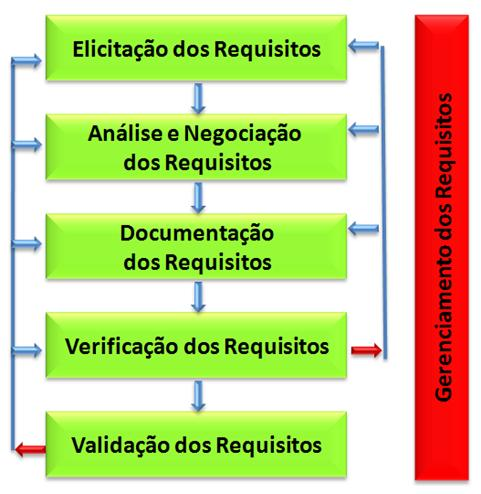
\includegraphics[width=5cm,height=5cm\textwidth]{figuras/requisitos}
     \caption{Gerenciamento de Requisitos}
     \end{figure}
    \end{columns}
  \end{frame}
\end{document}
